\epigraph{If you drive a car, it makes little difference what brand it is: all cars are driven
in essentially the same way. The same applies to computers. If you have a
Windows PC, the user interface won’t be affected by your computer hardware.
This is definitely not the case for industrial robots.}{\textit{Albert Nubiola \\ CEO at RoboDK}}

\section{RoboDK overview}

RoboDK (short for Robot Development Kit) is a development platform for industrial robot offline programming and simulation for industrial robots.

\subsection{RoboDK history}

RoboDK (the company) was founded by Albert Nubiola and Lauren Ierullo in January 2015 as a spin-off company from the \href{https://en.etsmtl.ca/unites-de-recherche/coro/accueil?lang=en-CA}{CoRo laboratory}   at ETS University in Montreal, Canada. RoboDK is a commercial version of RoKiSim, a multiplatform educational software tool for 3D simulation of serial 6-axis robots.

\subsection{RoboDK features}


The following section highlights some of the features RoboDK has to offer. 


\begin{itemize}
\item Intuitive graphical user interface
\item Drag-and-drop functionality 
\item Supported 3D models - Importing objects and creating new tools using 3D files such as STL, STEP and IGES
\item External axes - Integrating external axes to extend the robot’s reachability
\item Generating Programs - Generating programs for various robot manufacturers
\item Running programs on the fly – Executing programs directly from an external computer
\item Real-time monitoring – Viewingthe robot state on an external computer 
\item CAM for robots - converting 5-axis CNC toolpaths to robot programs and using a robot like a 5-axis CNC
\item Automated path solving - Avoiding robot errors, including singularities, joint limits, reach limits, and collisions
\item Fast collision detection - Defining the object interactions 
\item Advanced use - Creating robot programs from an external computer using a higher programming language. The RoboDK API is available in Python, C#, Visual Basic, C++, and Matlab
\item Simulating 2D vision cameras - Testing image recognition algorithms in the simulation environment
\item Multiple robot simulation - Synchronizing and programming multiple robots and moving them at the same time 
\item Customizable post processor - Integrating specific sensors or actuators such as grippers, force control, image processing, etc.
\end{itemize}

\subsection{RoboDK licences and versions}

RoboDK offers a free (limited), educational or professional version. 
The software is available for Windows, Mac OS, Ubuntu Linux or Android. It supports either 32 or 64-bit versions of the abovementioned operating systems. At the time of writing this document, the latest version of RoboDK is 5.2. The complete RoboDK revision history is available online at this \href{https://en.etsmtl.ca/unites-de-recherche/coro/accueil?lang=en-CA}{link}. The logo of RoboDK is shown in Figure \ref{fig:robodklogo}.

\begin{figure}[h]
    \centering
    
\includegraphics[width=0.6\linewidth]{img/robodk_logo.png}
    \caption{RoboDK logo.}
    \label{fig:robodklogo}
\end{figure}

\section{RoboDK robot library}

RoboDK supports offline programming and has an extensive robot library supporting many robot controllers, including:

\begin{itemize}
    \item ABB RAPID (mod/prg)
    \item Fanuc LS (LS/TP)
    \item KUKA KRC/IIWA (SRC/java)
    \item Motoman Inform (JBI)
    \item Universal Robots (URP/script)
\end{itemize}

The RoboDK library can be accessed either online via this \href{https://en.etsmtl.ca/unites-de-recherche/coro/accueil?lang=en-CA}{link}  or in the RoboDK application itself. 



\section{RoboDK interface}

The interface of RoboDK consists of the main menu, the toolbar, the station tree, the status bar, and the 3D view. A picture of the RoboDK interface is shown in Figure \ref{fig:robodkinterface}. An extensive documentation for RoboDK is available online via this \href{https://robodk.com/doc/en/Basic-Guide.html#Start}{link}.

\begin{figure}[h]
    \centering
    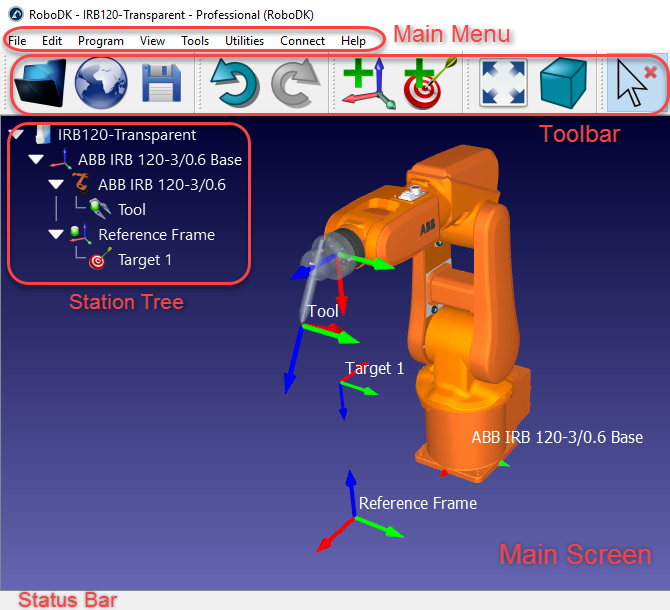
\includegraphics[width=0.9\linewidth]{img/robodk_interface.png}
    \caption{RoboDK interface v 5.0 running on Windows 10.}
    \label{fig:robodkinterface}
\end{figure}

\section{RoboDK API}

RoboDK provides a GUI to simulate and program industrial robots. No programming experience is required to simulate and program robots using the GUI. Unfortunately, the GUI has some limitations for simulation and offline programming. Then the RoboDK API can extend the capabilities of RoboDK using a programming language such as Python.

The API exposes a set of routines and commands to RoboDK, enabling the user to program the robot using high-level programming languages. The RoboDK API is available for Python, C#, C++, Visual Basic (.NET) and Matlab. Any of these programming languages can be used to simulate and program any robot arm. The API can conveniently handle the following tasks:

\begin{itemize}
    \item Automating the simulation
    \item Offline programming
    \item Online Programming
\end{itemize}

The RoboDK API is divided into the following modules:


\begin{itemize}
    \item robolink module - this module represents the link between RoboDK and the programming language
    \item Item module - any item from the RoboDK item tree can be retrieved.  An item can be a robot, a reference frame, a tool, an object or a specific project.
    \item robodk module - a module with a robotics toolbox for pose operations.All post processors depend on the robodk module.
\end{itemize}

\section{RoboDK Plug-Ins}

\subsection{RoboDK Plug-In interface}

Plug-Ins can extend RoboDK's functionality. Plug-Ins can be developed by using the RoboDK Plug-In interface. The RoboDK Plug-In interface is linked natively to the core of RoboDK. Examples of RoboDK Plug-Ins are available at this \href{https://github.com/RoboDK/Plug-In-Interface}{link}. 

\subsection{RoboDK Plug-In for SolidWorks}

\begin{figure}[h]
    \centering
    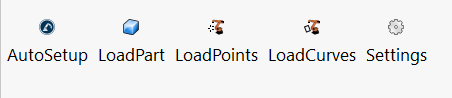
\includegraphics[width=0.6\linewidth]{img/solidworks_toolbar.PNG}
    \caption{SolidWorks RoboDK Plug-In Toolbar.}
    \label{fig:solidworkstoolbar}
\end{figure}


Solidworks is a professional 3D CAD modelling application. The RoboDK Add-in for SolidWorks allows to combine SolidWork's 3D CAD modelling features with RoboDK for robot simulation and offline programming and considerably simplifies the programmer's workflow. The programmed can load 3D models created in SolidWorks directly to RoboDK. Groups of curves and point can also be loaded to RoboDK, and robot programs can be generated from them.

\subsubsection*{SolidWorks RoboDK Plug-In Toolbar}

After opening SolidWorks under the RoboDK toolbar, the RoboDK Add-in presents the user five buttons. The RoboDK Plug-In for SolidWorks is shown in Figure  \ref{fig:solidworkstoolbar}. 

\begin{itemize}
    \item Auto Setup - the user selects the geometry (curves and points) and the model and the curves automatically to RoboDK.
    \item Load Part - only loads the 3D model from SolidWorks to RoboDK without the curves or points
    \item Load Point(s) - loads points to RoboDK as a new object. Selected surfaces are be used to calculate curve normals. 
    \item Load Curve(s) -  loads curves selected in RoboDK as a new item. Selected surfaces are be used to calculate curve normals. 
    \item Settinngs - opens default Settings window
\end{itemize}

\section{RoboDK post processors}

Post processors generate robot programs for robot controllers from the RoboDK simulation. Post processors are essential for offline programming of robots. A post processor defines the vendor-specific rules a robot program must follow. A robot is linked to a post processor in RoboDK. The post processors available in RoboDK by default are in this \href{https://robodk.com/doc/en/Post-Processors.html#AvailablePosts}{link}.  
A post processor in RoboDK is a Python script (.py extension). All the post processors of RoboDK are located in the
\mintinline{shell-session}{C:/RoboDK/Posts/} folder running on the Windows operating system.  To use a post processor it must be placed in the \mintinline{shell-session}{C:/RoboDK/Posts/} folder. The user can modify an existing post processor or create a new one from scratch. Modifications of post processors are described in \autoref{chap:implementation} in more detail. 